\documentclass{beamer}
\usetheme{Boadilla}

% Additional packages
\usepackage{graphicx}
\usepackage{amsmath}
\usepackage{booktabs}
\usepackage{hyperref}
\usepackage{natbib}
\usepackage{multirow}
\newcommand{\lowrank}{Natural GaLore}

\AtBeginSection[]{
  \begin{frame}
  \vfill
  \centering
  \begin{beamercolorbox}[sep=8pt,center,shadow=true,rounded=true]{title}
    \usebeamerfont{title}\insertsectionhead\par%
  \end{beamercolorbox}
  \vfill
  \end{frame}
}

\AtBeginSubsection[]{
    \begin{frame}
        \vfill
        \centering
        \begin{beamercolorbox}[sep=8pt,center,shadow=true,rounded=true]{title}
          \usebeamerfont{title}\insertsubsectionhead\par%
        \end{beamercolorbox}
        \vfill
        \end{frame}
}

\title[Natural GaLore]{Natural GaLore: A Memory Efficient Approach for LLM Training and Fine-tuning}
\author{Arijit Das}
\date{\today}

\begin{document}

\begin{frame}
    \titlepage
\end{frame}

\begin{frame}{Outline}
    \tableofcontents
\end{frame}

% TODO: Change the slide footer to show the section and subsection titles
% Part 1: Set clear context and define the problem
\section{Introduction}

\begin{frame}{Advanced Agentic Systems (AAS)}
    \begin{itemize}
        \item Since GPT-3 \citep{brownLanguageModelsAre2020}, the concept of in-context learning has made LLMs extremely flexible and powerful.
        \item This has opened the door to build AAS that can respond to a wide variety of queries and solve complex problems, which may require a combination of: knowledge, reasoning, compute and action.
        \item However, building reliable AAS for practical applications remains challenging.
    \end{itemize}
\end{frame}

\begin{frame}{Optimizing AAS}
    \begin{itemize}
        \item Solving such a complex problem requires systemically breaking it down into modules.
        \item Each module or agent is a call to an LLM which performs a subtask, requiring its own set of prompts and parameters.
        \item These modules can then be combined together as a directed graph, which solves the problem.
        \item Building realiable and robust AAS hence requires good prompt and parameter optimization techniques.
    \end{itemize}
\end{frame}

\begin{frame}{Prompt Optimization}
    \begin{itemize}
        \item Prompt optimization is the process of finding the optimal prompt for a given LLM to maximize performance on a specific task.
        \vspace{0.5em}
        \begin{itemize}
            \item \textbf{Prompt Proposal}: The challenge comes from the fact that they are inherently fuzzy and have a exponentially large solution space.
            \vspace{0.5em}
            \item \textbf{Credit Assignment}: Another issue is to find efficient ways of inferring how each prompt variable contributes to performance.
        \end{itemize}
        \item Algorithms like OPRO \citep{yang2024largelanguagemodelsoptimizers} and MIPRO \citep{opsahlong2024optimizinginstructionsdemonstrationsmultistage} approach this problem by building efficient prompt proposal sampling, and credit assignment mechanisms following ideas from Bayesian optimization.
    \end{itemize}
\end{frame}

\begin{frame}{Parameter Optimization}
    \begin{itemize}
        \item LLM training requires parameter optimization at three steps:
        \vspace{0.5em}
        \begin{itemize}
            \item Pre-training: The model is optimized for the Next Token Prediction task on vast amounts of raw natural language text data.
            \vspace{0.5em}
            \item Supervised Fine-tuning: Using high quality “Instruction Data”, the model is transformed from essentially an autocomplete model, into one which can perform in context learning.
            \vspace{0.5em}
            \item Preference optimization: Here responses are sampled, ranked according to user preferences and then the model is updated to prefer those.
        \end{itemize}
    \end{itemize}
\end{frame}

\begin{frame}{AAS Optimization}
    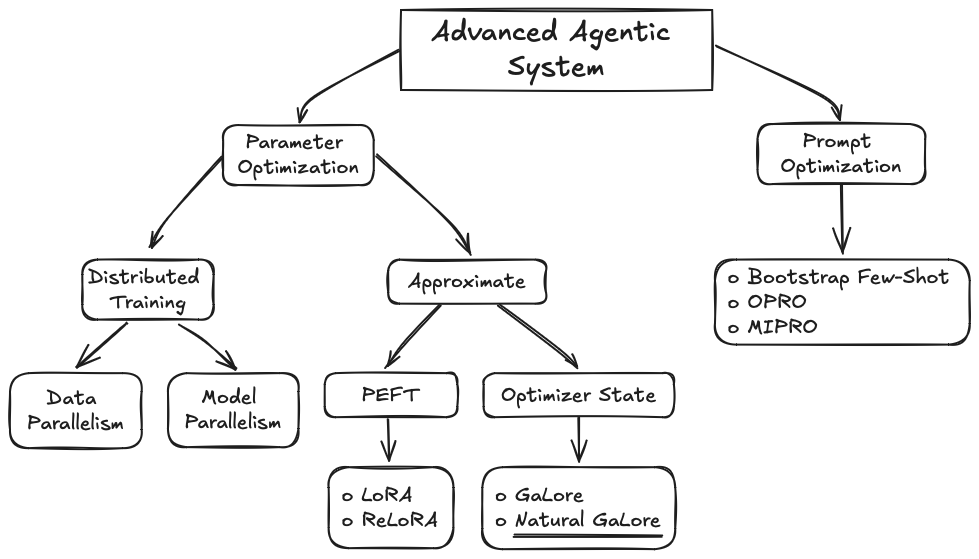
\includegraphics[width=\textwidth]{figures/AAS Optimization.png}
    \begin{itemize}
        \item In this work, I focus on the parameter optimization problem
    \end{itemize}
\end{frame}

% Part 2: Describe the options considered for solving the problem
\section{Parameter Optimization}

\begin{frame}{Next Token Prediction}
    \begin{itemize}
        \item LLMs are trained to predict the next token based on previously observed tokens (causal prediction).
        \item Given tokens \( x_{<t} = (x_1, x_2, \dots, x_{t-1}) \) the model is trained to maximize the probability of the next token \( x_t \)
    \end{itemize}
    \begin{equation}
        \text{Prob}_{\mathbf{\theta}}(x) = \prod_{t=1}^{T} \text{Prob}_{\mathbf{\theta}}(x_t \mid x_{<t})
    \end{equation}
\end{frame}

\begin{frame}{Objective: Negative Log-Likelihood (NLL)}
    \begin{itemize}
        \item The training objective is to minimize NLL:
    \end{itemize}
    \begin{equation}
        \Phi(\mathbf{\theta}) = -\sum_{t=1}^{T} \log \text{Prob}_{\mathbf{\theta}}(x_t \mid x_{<t})
        \label{eq:cross_entropy_loss}
    \end{equation}
    \begin{itemize}
        \item Penalizes low probability assignments to correct tokens.
        \item However is a high-dimensional, non-convex optimization problem.
    \end{itemize}
\end{frame}

\begin{frame}{Adam Optimizer}
    \begin{itemize}
        \item Adam \citep{kingmaAdamMethodStochastic2014} is an iterative stochastic gradient descent algorithm with adaptive learning rates and momentum
        \[
            \mathbf{\theta}_{k+1} = \mathbf{\theta}_{k} - \eta \mathbf{u}_{k}^{*}
        \]
        where \(\mathbf{g}_{k} = \nabla_{\mathbf{\theta}} \Phi(\mathbf{\theta}_{k})\) and \(\eta\) is the learning rate.
        \vspace{0.5em}
        \item The optimal update direction is determined using the momentum term \(\mathbf{m}_{k} \in \mathbb{R}^{r\times m}\) and the second moment estimate \(\mathbf{v}_{k} \in \mathbb{R}^{r\times m}\). With all operations being elementwise, the update direction becomes:
    \end{itemize}
    \begin{eqnarray}
        \mathbf{m}_{k} &=& \beta_{1} \mathbf{m}_{k-1} + (1-\beta_{1}) \mathbf{g}_{k} \\
        \mathbf{v}_{k} &=& \beta_{2} \mathbf{v}_{k-1} + (1-\beta_2) \mathbf{g}^{2}_{k}  \\
        \mathbf{u_{k}^{*}} &=& \mathbf{m}_{k} / \sqrt{\mathbf{v}_{k} + \epsilon}
        \label{eq:adam_update}
    \end{eqnarray}
\end{frame}

\begin{frame}{Memory Challenges}
    \begin{itemize}
        \item Training and fine-tuning LLMs demand enormous computational resources and are highly memory-intensive.
        \item Memory requirements: 
        \begin{itemize}
            \item Stem from storing billions of parameters, gradients, and optimizer states.
            \vspace{0.5em}
            \item For example for pre-training a Llama-7B model using Adam, requires 72GB of memory: 14GB for parameters and gradients each, 42GB for optimizer states and 2GB for activations.
            \vspace{0.5em}
            \item These limit the ability to train large models on hardware with limited memory capacity.
            \vspace{0.5em}
            \item Increase training costs and environmental impact.
        \end{itemize}
        \item \textbf{Objective}: Develop a memory-efficient approach for training and fine-tuning LLMs without sacrificing performance.
    \end{itemize}
\end{frame}

\begin{frame}{Distributed Training Techniques}
    \begin{itemize}
        \item \textbf{Data Parallelism}
            \begin{itemize}
                \item DDP combines data parallelism with efficient gradient synchronization.
                \item \textbf{Pros}: Efficient gradient updates, good scalability.
                \item \textbf{Cons}: Memory bottlenecks persist when model size exceeds single GPU capacity.
            \end{itemize}
        \item \textbf{Model Parallelism}
            \begin{itemize}
                \item Partitions model across multiple devices.
                \item Techniques: Pipeline parallelism \citep{huangGPipeEfficientTraining2019}, Tensor parallelism \citep{shoeybiMegatronLMTuningScaling2019}, Fully Sharded Data Parallel (FSDP) \citep{zhaoExtendingTorchElasticStateful2020}.
                \item \textbf{Pros}: Allows training of models larger than a single GPU.
                \item \textbf{Cons}: Communication overhead, complex implementation.
            \end{itemize}
    \end{itemize}
\end{frame}

\begin{frame}{Distributed Training Techniques}
    \begin{itemize}
        \item Data and Model Parallelism can be augmented with further techniques to reduce memory usage.
        \vspace{0.5em}
        \begin{itemize}
            \item \textbf{Gradient Checkpointing} \citep{chenTrainingDeepNets2016}
            \begin{itemize}
                \item Stores subset of activations during forward pass.
                \item Recomputes activations during backward pass.
                \item \textbf{Pros}: Reduces memory usage.
                \item \textbf{Cons}: Increases computational overhead.
            \end{itemize}
            \vspace{0.5em}
            \item \textbf{Memory Offloading}
            \begin{itemize}
                \item Moves optimizer states and gradients to CPU memory.
                \item Techniques: ZeRO-Offload \citep{rajbhandariZeROMemoryOptimizations2020}.
                \item \textbf{Pros}: Significant memory reduction.
                \item \textbf{Cons}: Increased system complexity, operational costs.
            \end{itemize}
        \end{itemize}
    \end{itemize}
\end{frame}

\begin{frame}{Parameter-Efficient Fine-Tuning (PEFT)}
    \begin{itemize}
        \item \textbf{LoRA (Low-Rank Adaptation)} \citep{huLoRALowRankAdaptation2021}
            \begin{itemize}
                \item Reparameterizes weight matrices using low-rank adapters
                \begin{equation}
                    W = W_0 + BA, \quad B \in \mathbb{R}^{n \times r}, A \in \mathbb{R}^{r \times m}
                \end{equation}
                \item \textbf{Pros}: Reduces trainable parameters, lowers memory usage
                \item \textbf{Cons}: May not match full fine-tuning performance, especially on complex tasks \citep{xiaChainLoRAEfficient2024}.
            \end{itemize}
        \vspace{0.5em}
        \item \textbf{ReLoRA} \citep{lialinReLoRAHighRankTraining2023}
            \begin{itemize}
                \item Extends LoRA for pre-training.
                \item Periodically updates frozen weights using learned adapters.
                \item \textbf{Pros}: Enables continual learning with lower memory.
                \item \textbf{Cons}: Requires initial full-rank training phase.
            \end{itemize}
    \end{itemize}
\end{frame}

\begin{frame}{GaLore: Gradient Low-Rank Approximation}
    \begin{itemize}
        \item Exploits low-rank structure of gradients to approximate optimizer states \citep{zhao2024galore}.
        \item The gradients \(\mathbf{g} \in \mathbb{R}^{n \times m}\) are projected onto a low-rank form using SVD: \(\mathbf{g} = \mathbf{P} \Sigma \mathbf{Q}^{T}\)
        \begin{equation}
            \mathbf{g}^{\text{low-rank}} = \mathbf{P}^{T} \mathbf{g}, \quad \mathbf{P} \in \mathbb{R}^{n \times r}
        \end{equation}
        \item Then after applying Adam to \(\mathbf{g}^{\text{low-rank}}\) the full parameter update is reconstructed by applying \(\mathbf{P}\).
        \item \textbf{Pros}:
            \begin{itemize}
                \item Significant memory reduction (up to 30\% compared to LoRA).
                \item Full-parameter updates, maintaining model capacity.
            \end{itemize}
        \item \textbf{Cons}:
            \begin{itemize}
                \item Performance may not match full optimizer state methods.
                \item Low-rank approximation may not capture full optimization dynamics.
            \end{itemize}
    \end{itemize}
\end{frame}

% Part 3: Describe the proposed approach
\section{Natural GaLore}

\begin{frame}{Natural GaLore: Proposed Approach}
    \begin{itemize}
        \item \textbf{Goal}: Accelerating convergence of GaLore to bridge the gap with full state optimizers like Adam and AdamW.
        \item \textbf{Key Idea}: Incorporate second-order information into the low rank projected gradients using the Fisher Information Matrix (FIM) to efficiently estimate natural gradients.
    \end{itemize}
\end{frame}

\begin{frame}{Low-Rank Gradient Descent in GaLore}
    \begin{itemize}
        \item GaLore restricts updates to an affine subspace defined by its principle components \(\mathbf{P}_k \in \mathbb{R}^{n \times r}\):
        \[
            \mathbf{u}_k \in \mathbf{\theta}_k + \text{Range}(\mathbf{P}_k)
        \]
        \item Then the second-order Taylor series expansion of the loss function along this subspace is:
        \[
            \Phi(\mathbf{\theta}_k + \mathbf{P}_k \mathbf{u}_k) \approx \Phi(\mathbf{\theta}_k) + \mathbf{g}_{k}^{\text{low-rank} T} \mathbf{u}_k + \frac{1}{2} \mathbf{u}_k^T \mathbf{H}_k \mathbf{u}_k
        \]
        where \(\mathbf{g}_{k}^{\text{low-rank}} = \mathbf{P}_k^T \nabla_{\mathbf{\theta}} \Phi(\mathbf{\theta}_k)\) is the projected gradient and \(\mathbf{H}_k = \mathbf{P}_k^T \nabla^2_{\mathbf{\theta}} \Phi(\mathbf{\theta}_k) \mathbf{P}_k\) is the local Hessian matrix.
    \end{itemize}
\end{frame}

\begin{frame}{Fisher Information Matrix}
    \begin{itemize}
        \item \textbf{Key idea}: When the loss function can be written in terms of the KL-divergence, the FIM approximates the Hessian matrix:
        \[
            \mathbf{F}_k = \mathbb{E}_{x \sim p_{\text{data}}} [ \mathbf{H}_k ]
        \]
        \item It captures the curvature of the loss landscape, enabling more efficient optimization.
        \item Natural gradient descent is Fisher efficient and reduces variance in gradient updates \citep{amariNaturalGradientWorks1998}:
        \[
            \text{Var}[\mathbf{\theta}_k] = \frac{1}{mk} \mathbf{F}_k^{-1}(\mathbf{\theta}_k^*) + \mathcal{O}\left(\frac{1}{k^2}\right)
        \]
        \item Smaller variance translates to faster convergence.
    \end{itemize}
\end{frame}

\begin{frame}{Natural Gradient Transform}
    \begin{itemize}
        \item In practice, FIM cannot be calculated efficiently.
        \item I approximate the empirical FIM using a mini-batch of \(h \approx 20\) samples:
        \[
            \mathbf{\hat{F}}_k = \frac{1}{h} \sum_{k=1}^{h} \mathbf{g}_{k}^{\text{low-rank}} \mathbf{g}_{k}^{\text{low-rank} T}
        \]
        \item The \textbf{natural gradient transform} can then be computed as:
        \[
            \mathbf{g}_k^* = \mathbf{\hat{F}}_k^{-1} \mathbf{g}_{k}^{\text{low-rank}}
        \]
        \item As with GaLore, after applying Adam to \(\mathbf{g}_k^*\) the full parameter update is reconstructed by applying \(\mathbf{P}\).
    \end{itemize}
\end{frame}

\begin{frame}{Natural GaLore Algorithm}
    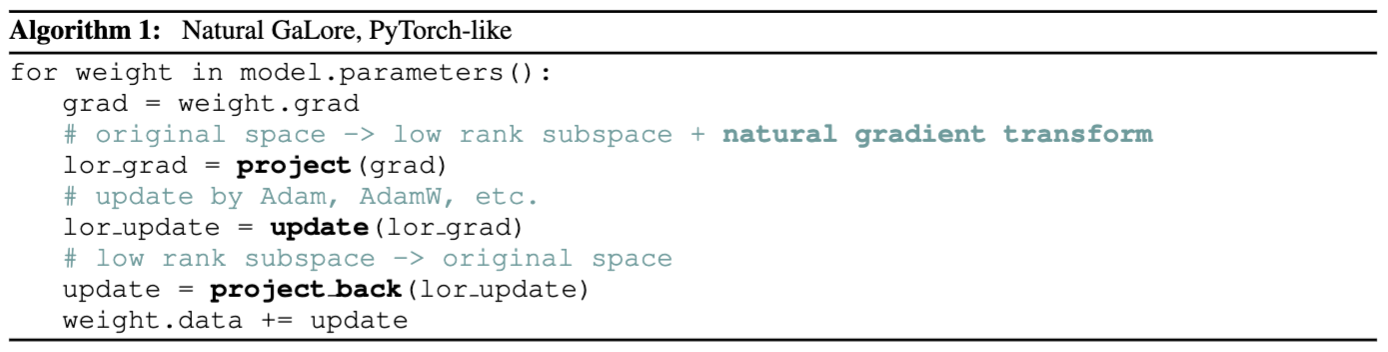
\includegraphics[width=\textwidth]{figures/natural_galore_algorithm.png}
    The algorithm combines low-rank projection from GaLore with efficient second-order updates.
\end{frame}

\begin{frame}{Natural Gradient Computation}
    \begin{itemize}
        \item Inverting the empirical FIM is computationally expensive.
        \item Here I use the Woodbury's Identity to compute the natural gradient efficiently:
            \begin{itemize}
                \item By re-writing \(\mathbf{\hat{F}}_k = \lambda I + GG^T\), I get:
                    \[
                    (\lambda I + GG^T)^{-1} = \frac{1}{\lambda} I - \frac{1}{\lambda^2} G (I + \frac{1}{\lambda} G^T G)^{-1} G^T
                    \]
                    where \(G = [\operatorname{vec}(\mathbf{g}_{k}^{\text{low-rank}}), \ldots, \operatorname{vec}(\mathbf{g}_{k-s}^{\text{low-rank}})]\) is the gradient history.
            \end{itemize}
        \item Can be computed using Cholesky Decomposition and matrix-vector products in \(\mathcal{O}(s^2)\) time:
                \[
                    S z = y, \quad S = I + \frac{1}{\lambda} G^T G
                \]
        \item Hence enabling scalable low-rank second order optimization.
    \end{itemize}
\end{frame}

\begin{frame}{Advantages of Natural GaLore}
    \begin{itemize}
        \item \textbf{Curvature Information}:
            \begin{itemize}
                \item Accounts for the geometry of the loss landscape.
                \item Enables more informed optimization steps in high-dimensional, non-convex spaces.
            \end{itemize}
        \item \textbf{Variance Reduction}:
            \begin{itemize}
                \item Natural gradients reduces variance in gradient estimates.
                \item Leads to faster convergence, especially in limited iterations.
                \item Further, when using a decaying learning rate schedule like with AdamW \citep{loshchilov2017decoupled}, the asymptotic convergence rate can be faster \citep{martens2020new} by a significantly large constant factor.
            \end{itemize}
        \item \textbf{Memory Efficiency}:
            \begin{itemize}
                \item Maintains low memory footprint, as with GaLore.
                \item Can be implemented without significant computational overhead.
            \end{itemize}
    \end{itemize}
\end{frame}

% Part 4: Experiments and Results
\section{Benchmarking Experiments}

\begin{frame}{Pre-training Experiments on C4 Dataset}
    \begin{itemize}
        \item \textbf{Models}: LLaMA variants with 60M, 130M, 350M, and 1.1B parameters.
        \item \textbf{Dataset}: C4 dataset.
        \item \textbf{Metrics}: Validation perplexity, memory consumption.
        \item \textbf{Results}:
            \begin{itemize}
                \item Our method achieves lower perplexity than GaLore across all model sizes.
                \item Closer performance to full optimizer state methods.
                \item Maintains significant memory savings.
            \end{itemize}
        \item \textbf{Conclusion}: Incorporating natural gradients accelerates convergence without significant additional memory overhead.
    \end{itemize}
\end{frame}

\begin{frame}{Pre-training Experiments on C4 Dataset}
    \begin{table}[ht]
        \centering
        \caption{\small{Comparison of Natural GaLore with other low-rank algorithms on pre-training various sizes of LLaMA models on the C4 dataset. Validation log perplexity is reported (averaged over 5 runs), along with a memory estimate (in gigabytes) of the total parameters and optimizer states based on BF16 format.}}
        \label{tab:lora_compare_llama}
        \resizebox{\linewidth}{!}{\begin{tabular}{lcccc}
        \toprule
                         & \textbf{60M} & \textbf{130M} & \textbf{350M} & \textbf{1.1B} \\
        \midrule
        Full-Rank        & 3.52 (0.36G) & 3.22 (0.76G) & 2.93 (2.06G) & 2.72 (7.80G) \\
        \midrule
        \textit{\lowrank} & \textbf{3.53} (0.24G) & \textbf{3.22} (0.52G) & \textbf{2.93} (1.22G) & \textbf{2.80} (4.38G) \\
        GaLore           & 3.56 (0.24G) & 3.24 (0.52G) & 2.95 (1.22G) & 2.90 (4.38G) \\
        Low-Rank         & 4.35 (0.26G) & 3.82 (0.54G) & 3.62 (1.08G) & 4.96 (3.57G) \\
        LoRA             & 3.55 (0.36G) & 3.52 (0.80G) & 3.24 (1.76G) & 2.96 (6.17G) \\
        ReLoRA           & 3.61 (0.36G) & 3.38 (0.80G) & 3.37 (1.76G) & 2.91 (6.17G) \\
        \bottomrule
        Rank $r / d_{\text{model}}$ & 128 / 256 & 256 / 768 & 256 / 1024 & 512 / 2048 \\
        Training Tokens  & 1.1B & 2.2B & 6.4B & 13.1B \\
        \bottomrule
        \end{tabular}}
    \end{table}
\end{frame}

\begin{frame}{Fine-Tuning on GLUE Benchmark}
    \begin{itemize}
        \item \textbf{Model}: RoBERTa-Base.
        \item \textbf{Benchmark}: GLUE tasks (CoLA, MRPC, STS-B, etc.).
        \item \textbf{Comparison} with LoRA, GaLore and full fine-tuning.
        \item \textbf{Results}:
            \begin{itemize}
                \item Comparable or better performance than LoRA.
                \item Achieved an average score of 86.05, close to full fine-tuning baseline of 86.28.
                \item Less memory consumption.
            \end{itemize}
        \item \textbf{Conclusion}: Effective for memory-efficient fine-tuning without signficantly sacrificing accuracy.
    \end{itemize}
\end{frame}

\begin{frame}{Fine-Tuning on GLUE Benchmark}
    \begin{table}[ht]
        \caption{\small{Evaluating Natural GaLore for memory-efficient fine-tuning on the GLUE benchmark using pre-trained RoBERTa-Base. We report the average score of all tasks. Memory consumption is reported in millions of parameters (M).}}
        \label{tab:fine_tuning}
        \centering
        \resizebox{\linewidth}{!}{%
        \begin{tabular}{l|c|cccccccc|c}
        \toprule
                   & \textbf{Memory} & \textbf{CoLA} & \textbf{STS-B} & \textbf{MRPC} & \textbf{RTE} & \textbf{SST-2} & \textbf{MNLI} & \textbf{QNLI} & \textbf{QQP} & \textbf{Avg} \\
        \midrule
        Full Fine-Tuning & 747M & 62.24 & 90.92 & 91.30 & 79.42 & 94.57 & 87.18 & 92.33 & 92.28 & 86.28 \\
        \midrule
        \textbf{\textit{\lowrank} (rank=4)} & 253M & 61.50 & \textbf{90.80} & \textbf{92.10} & \textbf{79.50} & \textbf{94.20} & \textbf{87.05} & \textbf{92.30} & 91.15 & \textbf{86.05} \\
        GaLore (rank=4) & 253M & 60.35 & 90.73 & 92.25 & 79.42 & 94.04 & 87.00 & 92.24 & 91.06 & 85.89 \\
        LoRA (rank=4) & 257M & \textbf{61.38} & 90.57 & 91.07 & 78.70  & 92.89 & 86.82 & 92.18 & \textbf{91.29} & 85.61 \\
        \midrule
        \textbf{\textit{\lowrank} (rank=8)} & 257M & 61.70 & \textbf{90.90} & \textbf{92.25} & \textbf{79.80} & \textbf{94.40} & \textbf{87.20} & \textbf{92.35} & \textbf{91.25} & \textbf{86.23} \\
        GaLore (rank=8) & 257M & 60.06 & 90.82 & 92.01 & 79.78 & 94.38 & 87.17 & 92.20 & 91.11 & 85.94 \\
        LoRA (rank=8) & 264M & \textbf{61.83} & 90.80 & 91.90 & 79.06  & 93.46 & 86.94 & 92.25 & 91.22 & 85.93 \\
        \bottomrule
        \end{tabular}
        }
        \vskip -0.1in
    \end{table}
\end{frame}

\section{Application: Fine-Tuning TinyAgents}

\begin{frame}{TinyAgent Framework}
    \begin{itemize}
        \item TinyAgent framework \citep{erdogan2024tinyagent} is an AAS for task-specific function-calling pipelines.
        \item \textbf{Goal}: Fulfill user queries through function-calling, respecting function interdependencies and passing correct arguments.
        \item \textbf{Key challenge}: Generating function-calling plans with correct functions, their arguments and interdependencies.
    \end{itemize}
\end{frame}

\begin{frame}{LLMCompiler for Function Calling}
    \begin{itemize}
        \item LLMCompiler \citep{kim2023llmcompiler} generates function-calling plans with required functions and arguments.
        \item It can then compile the plan into executable sequences.
        \item \textbf{Key challenge}: In the LLMCompiler paper, the authors had only experimented with 7B+ models. The question here is, if I could fine-tune smaller LLMs to generate a function plan with correct syntax, argument values, and respect for dependencies.
    \end{itemize}
\end{frame}

\begin{frame}{Challenges with Off-the-Shelf TinyLlama 1.1B}
    \begin{itemize}
        \item The off-the-shelf TinyLlama 1.1B (instruct-32k) performs poorly on function-calling tasks.
        \item Issues include:
        \begin{itemize}
            \item Incorrect function sets.
            \item Hallucinated function names.
            \item Incorrect or missing dependencies.
            \item Argument misplacement.
        \end{itemize}
    \end{itemize}
\end{frame}

\begin{frame}{Innoculation by Fine-Tuning}
    \begin{itemize}
        \item To solve this, I fine-tune TinyLlama 1.1B using the curated TinyAgent dataset \citep{erdogan2024tinyagent}.
        \item Fine-tuning enables the model to learn:
        \begin{itemize}
            \item Task-specific patterns for function-calling.
            \item Precise understanding of task dependencies and arguments.
        \end{itemize}
        \item Now there are three possibilities after fine-tuning:
        \begin{itemize}
            \item Performance improvement \(\implies \) pre-training/instruction tuning data of the model was weak for this task.
            \item No change in performance \(\implies \) the model doesn't have the capacity to learn this task.
            \item Otherwise, annotation artifact.
        \end{itemize}
    \end{itemize}
\end{frame}

\begin{frame}{TinyAgent Dataset: Overview}
    \begin{itemize}
        \item A meticulously curated dataset for building agentic systems on Apple MacBooks.
        \item Contains 40K examples of natural language queries and corresponding function-calling plans.
        \item Covers 16 distinct tasks such as:
        \begin{itemize}
            \item Email, Contacts, SMS, Calendar, Notes, Reminders.
            \item File Management, Zoom Meetings.
        \end{itemize}
        \item Dataset split:
        \begin{itemize}
            \item 38K training examples.
            \item 1K validation examples.
            \item 1K test examples.
        \end{itemize}
    \end{itemize}
\end{frame}

\begin{frame}{Fine-Tuning Strategy}
    \begin{itemize}
        \item During fine-tuning, the prompt includes:
        \begin{itemize}
            \item Descriptions of the ground-truth functions.
            \item Irrelevant functions serving as negative samples.
        \end{itemize}
        \item The model learns to select the correct functions rather than simply memorizing the ground truth.
        \item Several \textbf{in-context examples} are used to demonstrate how queries translate into function-calling plans.
        \item Examples are selected via RAG, leveraging a \textbf{DeBERTa-v3-small} model \citep{he2021debertav3} fine-tuned for multi-label classification to retrieve relevant examples from the training set.
    \end{itemize}
\end{frame}

\begin{frame}{Training Objective}
    \begin{itemize}
        \item The training objective is to maximize the \textbf{accuracy of generated function-calling plans}.
        \item Success is defined as:
        \begin{itemize}
            \item Correct function selection.
            \item Correct arguments.
            \item Correct order of function-calls.
        \end{itemize}
        \item Verifying the selection of the correct function set is straightforward: set comparison.
        \item Ensuring correct argument handling and order requires constructing the associated \textbf{Directed Acyclic Graph (DAG)}.
        \item DAGs check for equality in the structure and dependencies of the function-calls.
    \end{itemize}
\end{frame}

\begin{frame}{Fine-Tuning for Function Calling}
    \begin{itemize}
        \item \textbf{Task}: Function calling using TinyAgent framework.
        \item \textbf{Model}: TinyLlama 1.1B fine-tuned for 3 epochs, batch size 32, learning rate \(7 \times 10^{-5}\).
        \item \textbf{Dataset}: TinyAgent dataset with 40K examples.
        \item \textbf{Metrics}: Success rate in generating correct function-calling plans.
        \item \textbf{Results}:
            \begin{itemize}
                \item Our method achieves a success rate of \textbf{83.09\%}.
                \item Outperforms 16-bit LoRA (80.06\%) and GPT-4-turbo (79.08\%).
                \item Uses \textbf{30\% less memory}.
            \end{itemize}
        \item \textbf{Conclusion}: Enhances performance of smaller models, making them competitive with larger models.
    \end{itemize}
\end{frame}

\begin{frame}{Fine-Tuning for Function Calling}
    \begin{table}[ht]
        \vspace{-3mm}
        \caption{
        Latency, size, and success rate of TinyAgent models before and after quantization. Latency is the end-to-end latency of the function calling planner, including the prompt processing time and generation.}
        \label{table:t2}
        \centering
        \resizebox{\linewidth}{!}{%
        \begin{tabular}{c|c|c|c|c}
            \toprule
            Model &	Weight Precision &	Latency (seconds)	& Model Size (GB)	& Success Rate (\%) \\
            \midrule
            GPT-3.5 & Unknown & 3.2 & Unknown & 65.04 \\
            GPT-4-Turbo & Unknown & 3.9 & Unknown & 79.08 \\
            \midrule
            \multirow{2}{*}{TinyAgent-1.1B} & 16-bit (\textit{\lowrank}) & 3.9 & 2.2 & \textbf{83.09} \\
            & 16-bit (LoRA) & 3.9 & 2.2 & 80.06 \\
            \midrule
            \multirow{1}{*}{TinyAgent-7B} & 16-bit \citep{erdogan2024tinyagent} & 19.5 & 14.5 & 84.95 \\
            \bottomrule
            \end{tabular}
        }
        \vskip -0.1in
    \end{table}
\end{frame}

% Part 5: Conclusion
\section{Conclusion}

\begin{frame}{Conclusion}
    \begin{itemize}
        \item \textbf{Natural GaLore} is a memory-efficient approach for LLM training and fine-tuning which enhances GaLore by incorporating \textbf{natural gradients} for better performance.
        \item Its effectiveness was demonstrated through extensive experiments on pre-training and fine-tuning tasks.
        \item I also demonstrated practical benefits in Advanced Agentic Systems.
    \end{itemize}
\end{frame}

\begin{frame}{Future Work}
    \begin{itemize}
        \item Explore \textbf{low-memory and structured projection matrices} for further memory efficiency.
        \item Conduct more extensive empirical evaluations on fine-tuning tasks in Advanced Agentic Systems.
        \item Inspire future research on \textbf{optimizer state approximation} for memory-efficient training.
        \item Make large-scale model training more accessible on consumer-grade hardware.
    \end{itemize}
\end{frame}

\begin{frame}{}
    \begin{center}
        Thank You! Questions?
    \end{center}
\end{frame}

\begin{frame}[allowframebreaks]{References}
    \small
    \bibliography{iclr_template/iclr2025_conference}
    \bibliographystyle{iclr_template/iclr2025_conference}
\end{frame}

\end{document}